\subsection{A5 School Environment Criterion}

The school has a safe, healthy, nurturing environment that reflects the school’s purpose and is characterized by respect for differences, trust, caring, professionalism, support, and high expectations for each student.

\subsubsection{Caring, Concern, High Expectations}

\indicator{The school demonstrates caring, concern, and high expectations for students in an environment that honors individual and cultural differences.}

\prompt{To what extent does the school demonstrate caring, concern, and high expectations for students in an environment that honors individual differences and is conducive to learning?}

\begin{findings}
CMIS demonstrates caring, concern, and high expectations for all community members in an environment that honors individual and cultural differences.

The Virtues Project was established at the elementary level in 2013 and is a globally recognized initiative used to inspire kindness, justice, and integrity in schools worldwide. It highlights ways for educators to use character virtues as a foundation to create safe, caring, and high performing learning communities. 

During 2015 the virtues were highlighted at the MS level during Health and Wellness classes, where they reviewed virtues and initiated \href{https://docs.google.com/forms/d/e/1FAIpQLScP9Fpphz10qaY0S4RO3VLKBQ54RC3WQdP-FGIBbPOcXzMwpQ/viewform?c=0&w=1}{random acts of kindness campaign}. At the beginning of the 2016-17 school year the virtues were acknowledged and practiced school-wide.

\minor{Examples}

In September 2016, middle and high school students focused on the monthly virtues of respect  and trust  which are essential  components for creating a caring and respectful environment that honors individual differences.

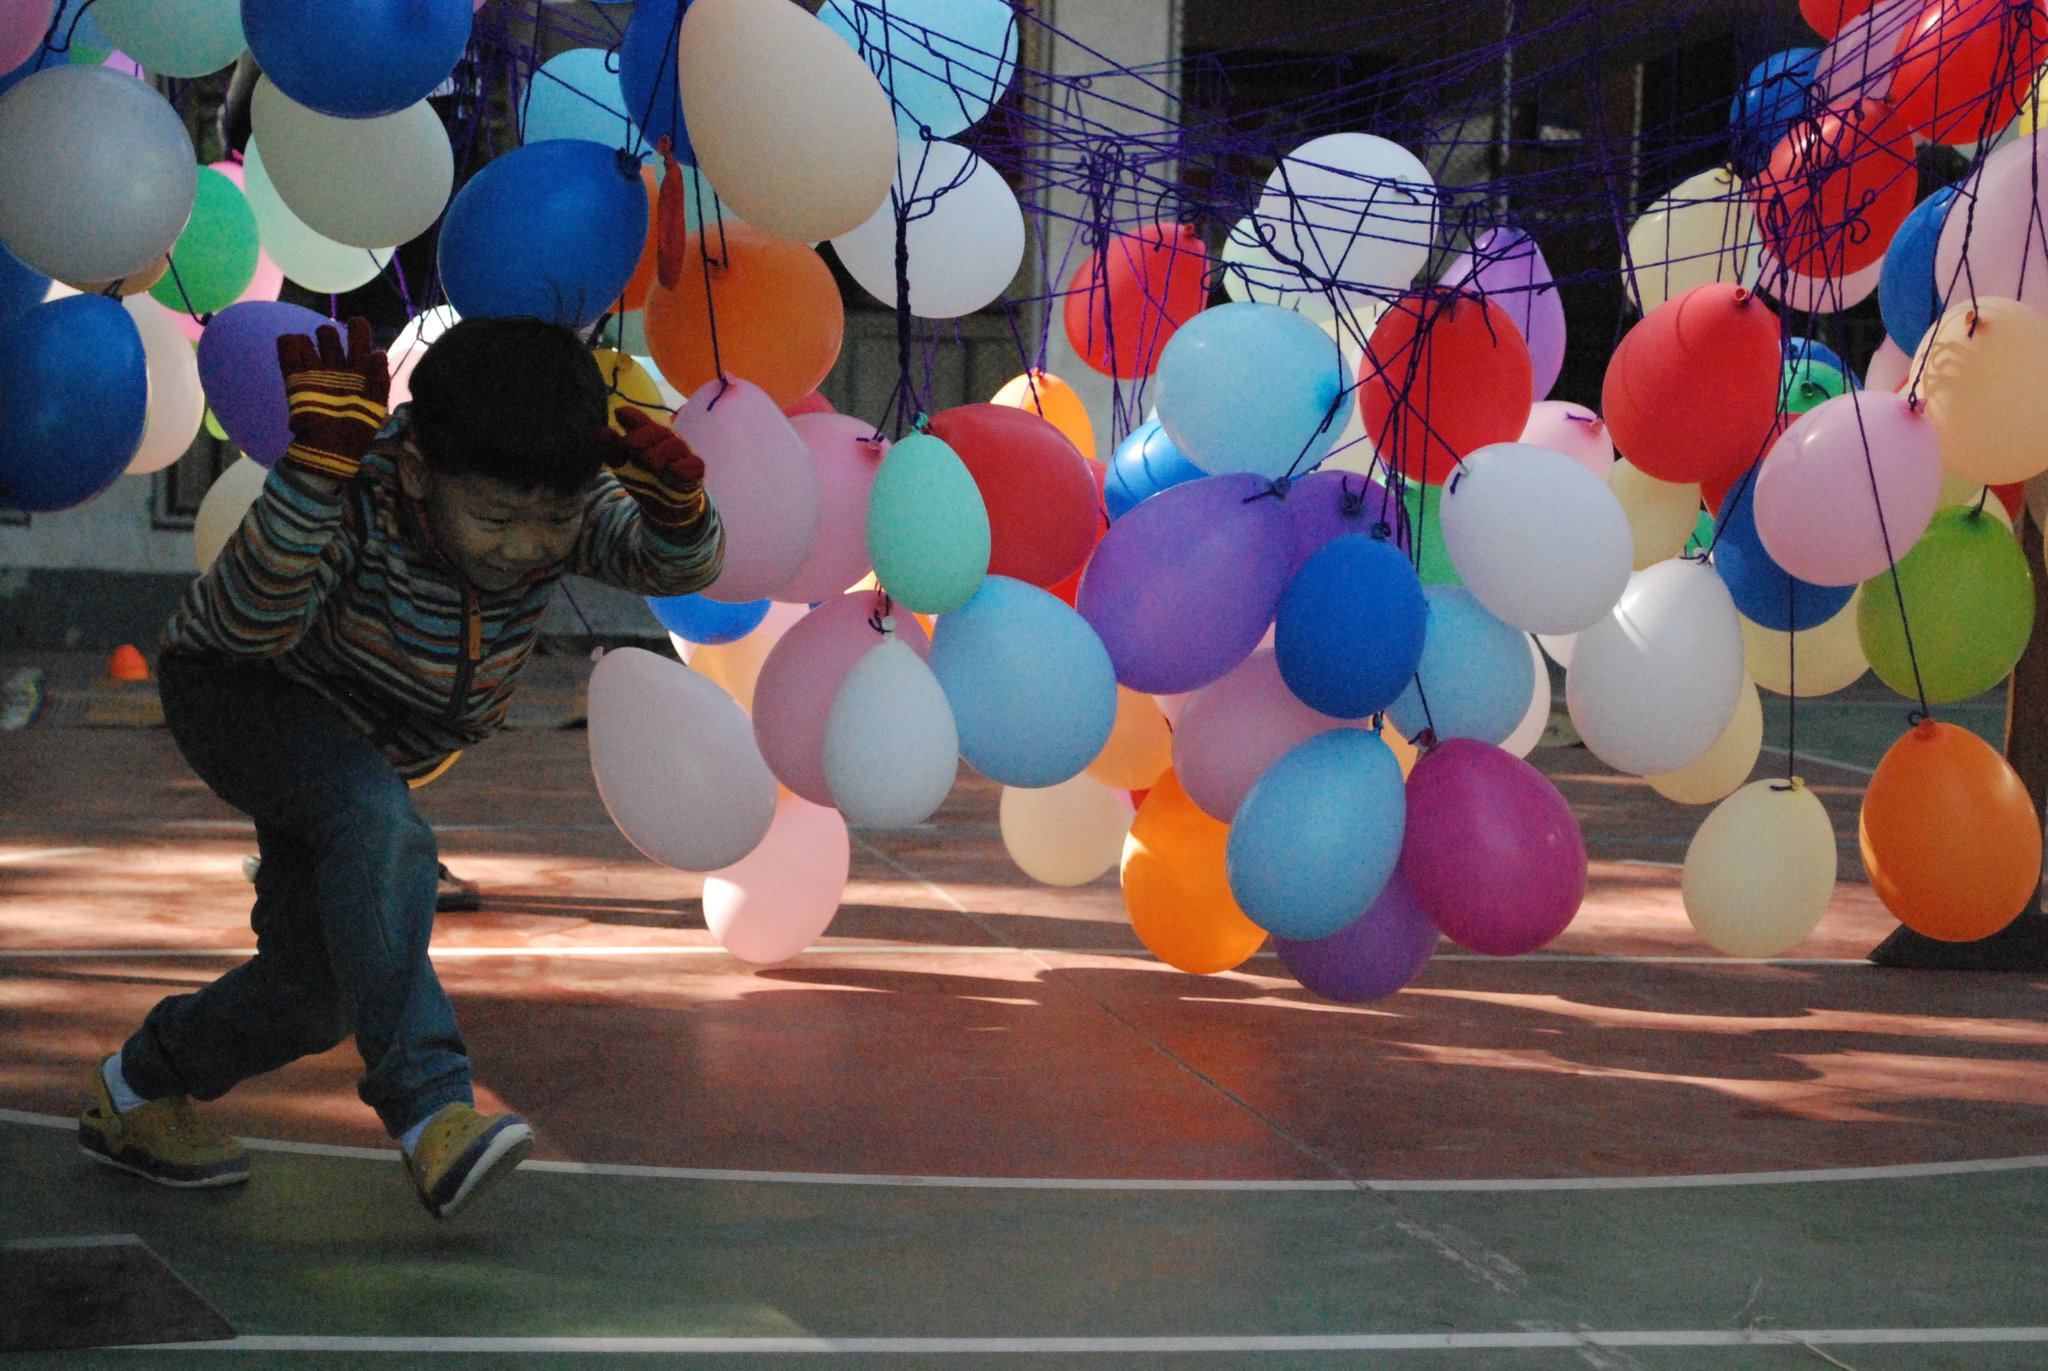
\includegraphics[width=\textwidth]{4_1_5_a.jpg}

In February 2017, the school counselors facilitated a school-wide \href{https://docs.google.com/a/cmis.ac.th/document/d/1PsHRple71FshloSGrqvYHgQQCYx9_CwCsbtlMAkb-Aw/edit?usp=sharing}{Great Kindness Challenge} (GKC) to highlight the monthly virtue of kindness.\href{https://dochub.com/roneldanelcapadona/gDPKV2/gkc?dt=ysuio255qfhtbryf}{ The Great Kindness Challenge} is a globally recognized, proactive and positive bullying prevention initiative that has been shown to improve school climate and increase student engagement. CMIS also used it as a fundraising opportunity to raise money for a local orphanage and as a meaningful way to promote the CMIS Virtues Project school-wide

\href{https://docs.google.com/a/cmis.ac.th/document/d/1Mv1xjTpbY36naur8SDt9GanKNfR7YtYVL-bWwGLPSHo/edit?usp=sharing}{Monthly Virtue Assemblies} at the elementary level are performed by each grade level and focus on the importance of each virtue and how they help CMIS to live harmoniously together. The Awesome Eagles Program was launched in the Fall of 2014 to foster teamwork and encourage CMIS elementary staff to recognize and reward students when they witness an act of kindness, cooperation, and empathy. The students work together to collect Eagle Bucks for their class. The grade level with the most Eagle  Bucks each month is announced at the Virtue Assembly after which they celebrate with a class trophy and an ice cream party.

Thai Day and \href{https://docs.google.com/a/cmis.ac.th/document/d/1YGCBI_uQVVcvOvw4c_Q2GcoJQzadFou1_6WtBAMTTaE/edit?usp=sharing}{International Day} are school-wide traditions that highlight the high expectations CMIS holds for all community members in terms of respecting global values and appreciating cultural differences. 

With the addition of a counselor position at the middle school level in 2014, CMIS now has a counselor available at each division: elementary, middle and high school. They are part of the CMIS Student Success Team and develop strategies with students, teachers, administrators, and parents to help students be academically, emotionally, and socially successful. Some of the ways they do this are by:

\begin{itemize}
\item Providing individual and small group counseling based on student needs
\item Working with students to develop effective organization, time management, and study habits
\item Helping students set realistic academic and career goals and develop a plan to achieve them
\item Teaching classes on topics such as bullying, parenting, health, and planning for college or careers after graduation.
\item Identifying and reporting possible cases of neglect or abuse
\item Referring students and parents to resources outside the school for additional support
\end{itemize}

With the addition of a Student Service Coordinator position in 2015, the \href{https://docs.google.com/a/cmis.ac.th/presentation/d/1sWhr1U3qZIGEu2aQdWOl0OQ5Rkd8iRGWmUlszEJLz2o/edit?usp=sharing}{CMIS Student Success team} was established. This team consists of the health officer, counselors, and the learning support teachers. They meet regularly to review student achievement,  safety and wellbeing. If teachers have concerns related to their students they are encouraged to reach out to the Student Success Team facilitated by the Student Service Coordinator. There is a \href{https://docs.google.com/a/cmis.ac.th/forms/d/e/1FAIpQLScVtFtaEXarGOjwsiJyGdbLAMbeNzG9m44i1fWXFLbtMKZcUg/viewform}{Student Service Request Form} available on the teacher dashboard section of the CMIS Handbook.This form activates immediate support from the team to meet with the teacher and create a plan of action.

\minor{So what...}

CMIS works hard to create a student centered environment that models genuine caring, concern, and high expectations for ALL. CMIS aims to always maintain an environment that honors individual differences and is conducive to learning. CMIS understands that a nurturing school climate is crucial for student learning and looks forward to finding additional ways to strengthen it.
\end{findings}

\subsubsection{Student Self-Esteem}

\indicator{The school fosters student self-esteem through high expectations for each student and recognition of successes.}

\prompt{To what extent does the school foster student self-esteem through high expectations for each student and recognition of successes?}

\begin{findings}
CMIS fosters student self-esteem through high expectations for ALL students and recognition of successes.
CMIS helps students to understand that self-esteem is how we value ourselves; it is how we perceive our value to the world and how valuable we think we are to others. The following are some outward student attributes of positive self-esteem that are described in our student learner outcomes and illustrated in our CMIS \href{http://cmis.ac.th/about/vision}{Vision Tree}. 

\begin{itemize}
\item Flexibility
\item Resilience
\item Courage
\item Self-direction 
\item An ability to make mistakes and learn from them 
\item An ability to accept mistakes from others 
\item An ability to solve problems 
\item An ability to trust others 
\end{itemize}

CMIS believes that publicly recognizing student’s thinking and accomplishments can benefit their learning and the overall school climate. It also believes that recognition needs to be authentic and meaningful.

Some examples are:
\begin{itemize}
\item Providing opportunities for students to voice their opinions (e.g. Stuco meetings with Superintendent, cafeteria student survey, communication group discussions etc.)
\item Weekly “shout outs” of students who have achieved outside of school on \href{http://blogs.cmis.ac.th/eagles/friday-september-16-2016/}{CMIS weekly announcements} (athletics, contests, performances etc)
\item\href{https://docs.google.com/a/cmis.ac.th/document/d/1DgY3NXB6m6qvmWnaRr2B2jswCGHRjaPFNPJA2Xzk1qw/edit?usp=sharing}{ Middle School Awards Assembly} for students that have demonstrated excellence in academics, athletics, the arts, and global citizenship
\item H\href{https://docs.google.com/document/d/1pxioSUeOgKZ4dT1jA9DiVzDjZjtrxuM-Gjqh7fRy0Us/edit?usp=sharing}{igh School Awards Evening} for students that have demonstrated excellence in leadership, academics, athletics, the arts, and global  citizenship.
\item ES and MS teachers recognize students of the month who have demonstrated resilience in their learning.
\item Student work is displayed on campus and on the website. 
\item Students encouraged to share their expertise by competing in local and international competitions (National History Day, MUN , poetry  etc.)
\end{itemize}

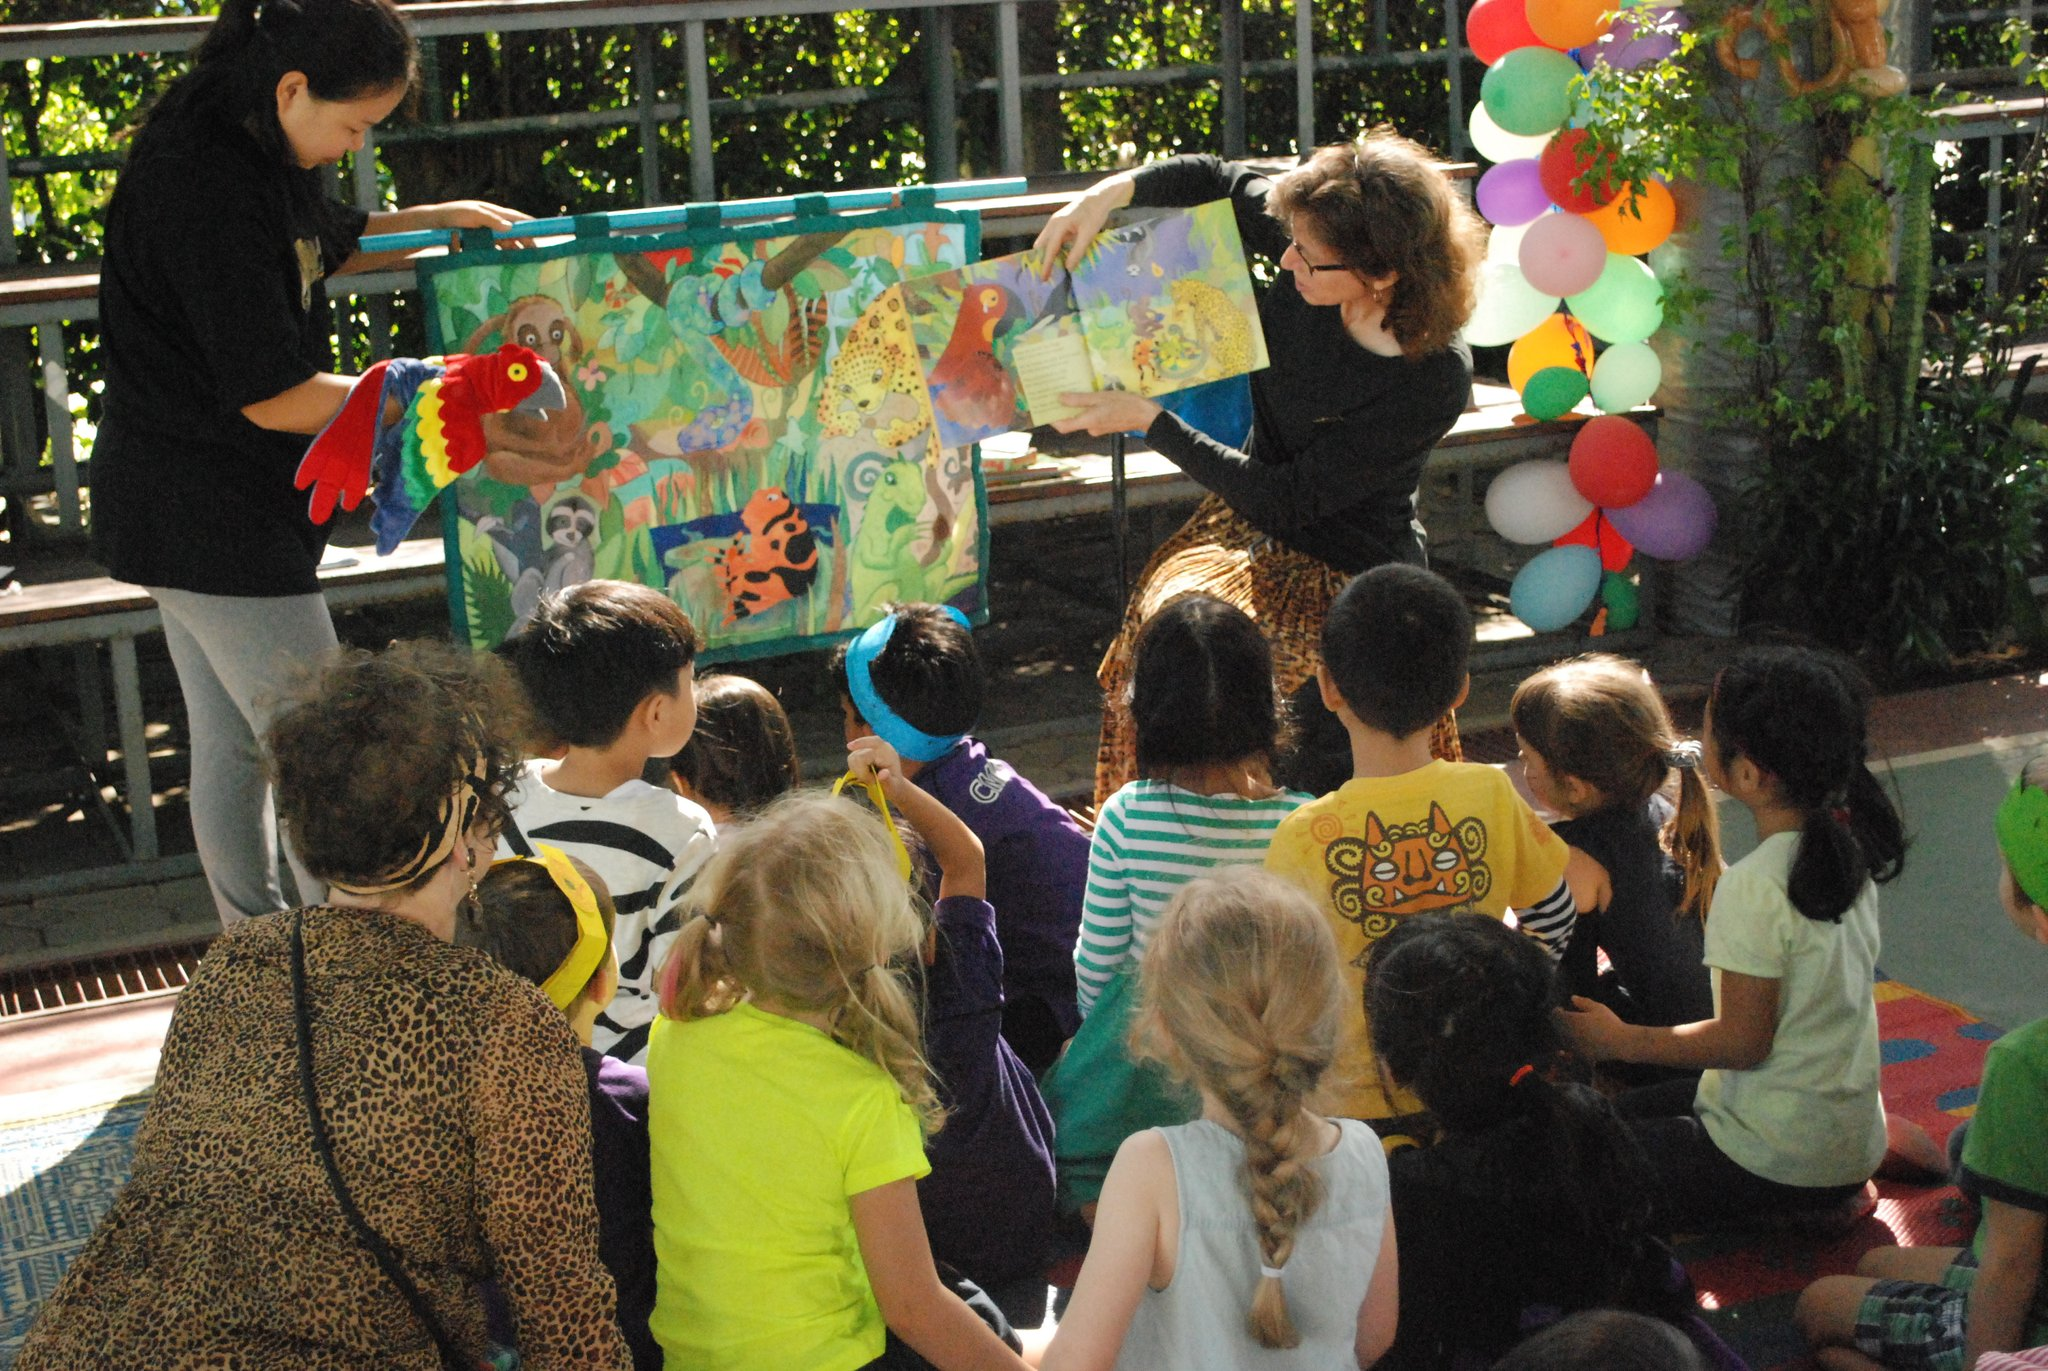
\includegraphics[width=\textwidth]{4_1_5_b.jpg}

\minor{So what}

CMIS works hard to foster student self-esteem through high expectations for each student and recognition of successes. It understands the importance of having opportunities for students to reflect on how positive self-esteem gives them the strength and flexibility to take charge of their lives and grow from their mistakes without the fear of rejection. CMIS will continue to find new ways to encourage positive student self-esteem and recognize student achievement. 
\end{findings}

{\centering\includegraphics[width=\textwidth]{chapter4_A5.jpg}}

\subsubsection{Mutual Respect and Communication}

\indicator{Mutual respect and effective communication among and between staff, students, and parents is evident. There is understanding of the importance of cross-cultural communication in improving teaching, learning, and management.}

\prompt{What evidence supports mutual respect and effective cross-cultural communication among and between staff, students, and parents?}

\begin{findings}
CMIS believes that cultural awareness is the key to effective cross-cultural communications. 

CMIS defines cultural awareness as the ability to empathize that a person's behaviors and reactions can be culturally driven and that while they may not match our own, they are culturally appropriate. It believes that acceptance of all CMIS community members is essential and standards for respectable behavior need to be regularly revisited. 

\minor{Examples}

\begin{itemize}
\item During staff meetings the following Norms of Conduct are reviewed at every meeting:
\item Be present (mindful)
\item Respect time
\item Be adaptive
\item Be true
\item Assume positive intent
\item Ground statements in evidence
\end{itemize}

During CMIS staff and parent meetings the Pluses and Delta protocol is used to elicit feedback from the meeting participants about the meeting effectiveness. By using Plus/Delta, CMIS teams can continuously improve meetings and show respect for people by discussing the value of or ability to improve the time spent together. Providing an opportunity for constructive criticism demonstrates attentive listening, and mutual respect--skills that CMIS want to model positively to all  students.

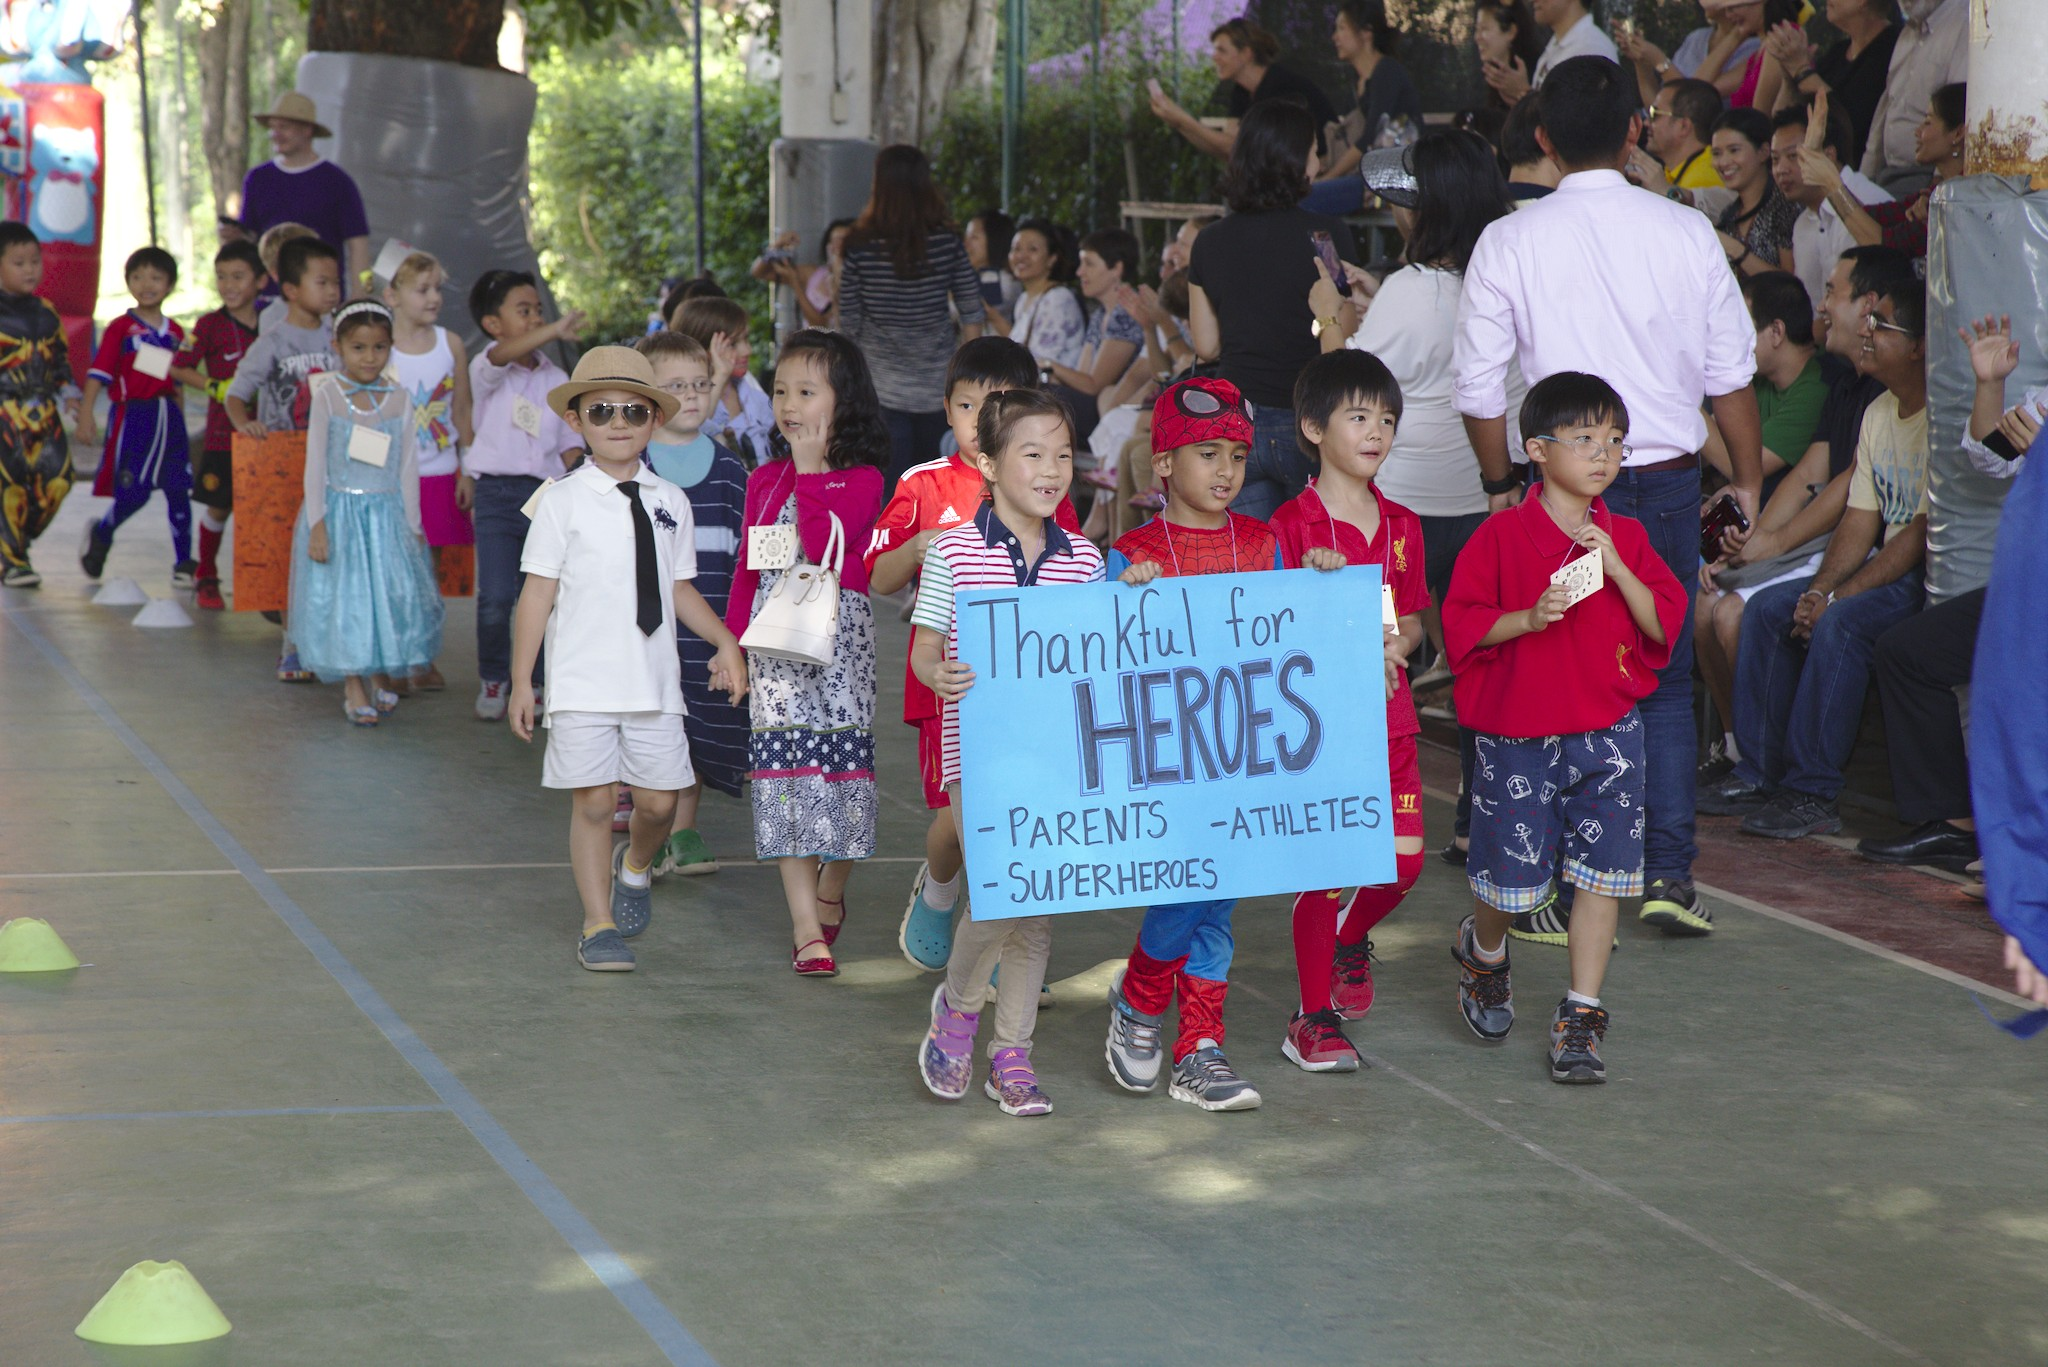
\includegraphics[width=\textwidth]{4_1_5_c.jpg}

When communicating with staff, students and parents the CMIS leadership tries to keep in mind that even though English is considered the international language of the school, the majority of the community who speak English are not native speakers.When communicating cross-culturally, CMIS makes particular efforts to keep communication clear, simple and unambiguous. It also ensures that translators are available at school events.

\minor{Examples}

There is a PTG meeting monthly that fosters communication between the parents and the school. Topics for discussion are \href{https://docs.google.com/a/cmis.ac.th/document/d/1kiwakkg8eKdtEexCxVNx-m1CfC3VqxhukDy8WXDPGKY/edit?usp=sharing}{parent generated}  and based on parent feedback. The school management and parent translators are always present for support.

Once a semester, there is a parent teacher conference where teachers, students, administrators, and parents come together and discuss the growth of their respective students. \href{https://docs.google.com/a/cmis.ac.th/document/d/1XA31w9WsFCzB3k9LcQnU46sTUmMeEiObDQ8yOqCPZdU/edit?usp=sharing}{CMIS National Honors Society} students are available as parent translators.

CMIS has a \href{https://docs.google.com/a/cmis.ac.th/document/d/1yZyHuHhAg7tHITOtlZQdX_w4kinRwL6J_Y_zco_7jSE/edit?usp=sharing}{Korean Liaison} fully devoted to communication across culture and language to Korean families.

\minor{So what...}

CMIS believes that mutual respect and effective communication among and between staff, students, and parents is crucial for a positive learning environment. It models cross-cultural communication to improve student achievement through teaching, learning, and management.
\end{findings}

\subsubsection{Teacher Support and Encouragement}

\indicator{There is a level of support and encouragement for teachers to use innovative approaches to enhance student learning.}

\prompt{How effective is the level of support and encouragement for teachers to use innovative approaches to enhance student learning?}

\begin{findings}
During CMIS professional development opportunities teachers learn different strategies to promote innovative teaching to enhance student learning.

\minor{Examples}

In 2015 CMIS hosted a region-wide workshop that focused on \href{https://docs.google.com/forms/d/e/1FAIpQLSdK2QvcDZyM_yfhT22BgModehhwhn3I8Ps6VoW2EIzaK-qing/viewform?c=0&w=1}{ Innovative Teaching and  ELL Learners} and invited educators from seven neighboring international schools to attend as well as all CMIS staff. 

In August 2016 all CMIS teacher received CMIS training on \href{https://docs.google.com/a/cmis.ac.th/presentation/d/1S1x1yEj7KDD6jM7u1RdTZJEt10_0r6mcJ-LmRb6iPWs/edit?usp=sharing}{Productive Failure}  based on the findings of Dr. Manu Kapur, Associate Professor of Curriculum, Teaching, and Head of Learning at Learning Sciences Lab in Singapore. CMIS teachers learned that productive failure affords better conceptual understanding, creative thinking, and helps students to transfer learning.

In November 2016 all CMIS all math teachers received research based training on \href{https://drive.google.com/a/cmis.ac.th/file/d/0ByVFfrm0zfolSXFEZFJVN1VOaTQ/view?usp=sharing}{Focus, Coherence, and Rigor in Math}: Reimagining Mathematics Instruction to Improve Access and Equity to all Students. The \href{https://docs.google.com/document/d/14wHOzYz9lk79YGv4aYLtMEkqAN0Z6vBBI3POYZPeIC4/edit?usp=sharing}{three day workshop} was sponsored by EARCOS and invited teachers from around Asia to attend. 

Each year CMIS teachers have a personal budget for professional development that encourages teachers to seek out their own learning, enrich their craft and enhance student achievement.

CMIS believes that providing teacher opportunities for self reflection in a safe, non threatening environment naturally promotes teacher innovation. In July, 2015 the \href{https://docs.google.com/document/d/15_5X5QtixmWVheEUBVO9N1aislsLDm_ZW4-4g4YQ7F4/edit?usp=sharing}{CMIS Teacher Observation Tool} was modified to a more coachable model that  focused on empowering the teacher to review and self reflect on instructional practice by reviewing observational data. Teacher feedback has indicated that they find the CMIS evaluation process to be meaningful and supportive,

``The teacher evaluation process we have in place at CMIS is comfortable and useful. Having discussed the framework ahead of time, I did not feel any nervousness or pressure that I have in past teaching positions when being evaluated. The feedback provided after my observation guided me to self-reflect and I was able to ask questions and see where I could focus my instruction to best assist my students.'' -CMIS Elementary Teacher

\minor{So what...}

CMIS will continue to foster teacher innovation by putting self-reflection, critical thinking, inquiry, and creative brainstorming at the center of CMIS professional development.

CMIS leadership is currently working with teachers to increase Project Based Learning. While most teachers have done projects, the majority do not use the defined set of methods associated with high-quality PBL. These methods include developing a focused question, using solid, well crafted performance assessments, allowing for multiple solutions, enlisting community resources, and choosing engaging, meaningful themes for projects.  (e.g, National History Day)
\end{findings}

\subsubsection{Safe, Clean, and Orderly Environment}

\indicator{The school has existing policies, regulations and uses its resources to ensure a safe, clean, and orderly place that nurtures learning, including internet safety.}

\prompt{Comment on your analysis of the effectiveness of a) the existing policies and use of resources to ensure a safe, clean, and orderly place that nurtures learning, and b) all aspects of the school with respect to safety regulations including effective operating procedures for internet safety.}

\begin{findings}
CMIS has several existing policies, regulations and uses its resources to ensure a safe, clean, and orderly environment that nurtures learning.

CMIS has a full time Health Officer as well as a fulltime nurse. The Health Officer provides a professional service utilizing knowledge and experiences in a caring and supportive manner to the students and staff in the promotion of health and well being. The Health Officer is in a unique position to provide the critical link between the school, students, teachers, administration, families, community and medical care. The health officer is part of the Student Success Team and promotes the optimal health status of students by: 
	 	 	
\begin{itemize}
\item Educating students through social and emotional health promotion classes.
\item Communicating relevant health alerts/promotion through the ‘CMIS Health Matters’ Newsletter. 
\item Promoting and assisting in the control of communicable diseases through monitoring immunization programs, early detection, surveillance, reporting and follow-up of contagious diseases.
\item Organizing and evaluating evacuation plans and lockdown procedures and implementation. 
\item Instructing in First Aid training and management of staff teams.
\item Implementing Individual Healthcare Plans for students with special health needs, including the administration of medication.
\item Overseeing school-wide health screening procedures (e.g. vision, body mass index, scoliosis) 
\item Coordinating between the school, parents and the cafeteria, lunch program, and healthy food choices.
\item Monitoring and assessing the air quality and heat index within Chiang Mai and facilitating decisions on any activity restrictions required. Sharing information with the community.
\item Participate in CMIS ‘Child Protection Committee’ to support and protect students from harm  or abuse. Keep Child Protection Handbook  for staff updated.
\item Monitoring Health and Safety within the school including playground safety, water quality, hygiene standards, and recording and acting upon any incidents reported at school. 
\end{itemize}

CMIS has a Child Protection Committee that includes the principals, health officer, counselors, student-service coordinator and superintendent. The committee members act as student advocates for the reporting of any social, emotional, or physical abuse of students.The committee created a \href{https://docs.google.com/a/cmis.ac.th/document/d/1NtJ-Yz1ra-dug9r6BmMGqTD3tE9TFxx5W1QhBzPYlxI/edit?usp=sharing}{Child Protection Manual} for staff that is available in the CMIS Faculty Handbook. In an effort to increase awareness and accountability, CMIS implemented a \href{https://docs.google.com/a/cmis.ac.th/forms/d/185Ul5UTdsOSC8btz8CWdIvklNYs6WdPdnzb7gUrOYyM/edit}{Child Protection Quiz} to all staff this year that reviewed the contents of the manual. It also included a \href{http://cmis.ac.th/about/employment}{Child Abuse Statement} to be advertised on the CMIS employment page and requires all permanent staff to complete a criminal background check prior to employment.

The school management team meets monthly to assess the structure and procedures in place to ensure a safe, clean, and orderly environment. The Assistant Manager is part of the management team and oversees the maintenance department. Staff are asked to assist in the the care and maintenance of school materials, equipment, and property by reporting any damage or safety concerns by completing a \href{https://docs.google.com/a/cmis.ac.th/forms/d/e/1FAIpQLSe3YhMowLuZm-HuEG2v_6M2HYfOmQJ5tQG5gB2nEAksooUQNA/viewform}{Job/Work Request Form} available on the school website.

The IT Department is committed to developing learners that can use information technology safely and effectively to improve their lives.To thrive as global citizens CMIS students need to be able to adapt to the rapid pace of technological change and leverage this to solve complex global problems.

The IT curriculum is aligned to the \href{https://www.csteachers.org/}{Computer Science Teachers Association standards} and is designed to integrate computer science fluency and competency. CMIS  aims to provide academic coherence to the rapid growth of computing and technology in the modern world, alongside the need for an educated public that can utilize that technology most effectively to the benefit of humankind.

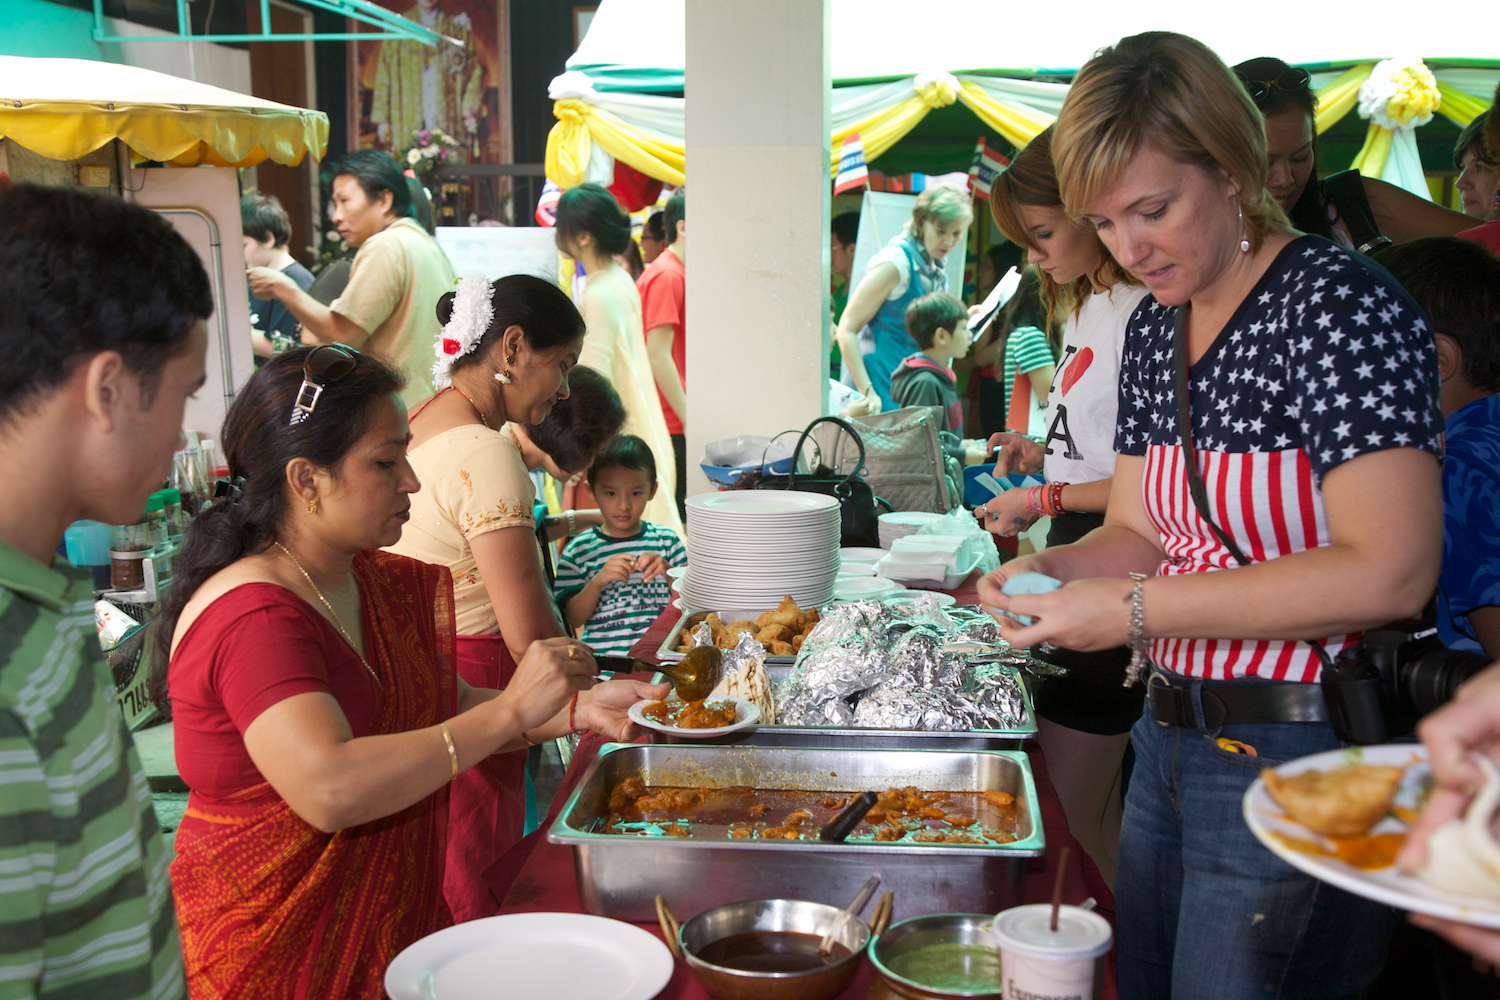
\includegraphics[width=\textwidth]{4_1_5_d.jpg}

The CMIS IT Department acts as the guiding resource for the CMIS community on digital safety and created the Acceptable Use Policy (AUP) that applies to all staff (including temporary staff), visitors, contractors, students, and guests of the school and to those using CMIS' IT resources.  CMIS definition of internet safety includes web services, chat rooms, bulletin boards, newsgroups, peer-to-peer file sharing and instant messaging software.  The IT Department also maintains the Email Acceptable Use Policy that applies to all users of CMIS IT resources including, but not limited to CMIS staff (including temporary staff), visitors, contractors, students and guests of the school.  

All of these policies are available in our student handbook available on the school website, in the CMIS Faculty Handbook and are communicated out regularly with the community through \href{https://docs.google.com/a/cmis.ac.th/presentation/d/1QRUmBmMM63pQlvP0Qemq272VPojLj5sZv3GuweO9J-Q/edit?usp=sharing}{presentations} and workshops.

\minor{So what...}

CMIS has worked hard to improve and strengthen existing policies, regulations and uses its resources to ensure a safe, clean, and orderly place that nurtures learning, including internet safety. 

Safety has always been a priority for CMIS but as with all initiatives, especially technology, procedures can become quickly outdated without regular evaluation and modification. With more streamlined practices in place, CMIS is committed to continuously bolstering the safety of our environment. 
\end{findings}

\subsubsection{Conclusions}
The findings suggest that CMIS addresses this criterion to a high degree. In an effort to increase student achievement further in this area CMIS plans to:

\minor{Maintain and Monitor}
\begin{itemize}
\item Structures for student care, respectful interactions, and campus/resource safety.
\item Communication and practice theses structures with the community
\end{itemize}
\minor{Investigate Better Practice}
\begin{itemize}
\item Additional (research based) ways for CMIS to continually update safety procedures.
\end{itemize}
